\documentclass[11pt, norsk]{article}
%\usepackage[latin1]{inputenc}
\usepackage[T1]{fontenc}
\usepackage[utf8]{inputenc}
\usepackage[norsk]{babel}   % S P R A A K


% \usepackage{graphicx}    % postscript graphics
\usepackage{amssymb, amsmath, amsthm, amssymb} % symboler, osv
\usepackage{mathrsfs}
\usepackage{url}
\usepackage{thmtools}
\usepackage{enumerate}  % lister $  
\usepackage{float}
\usepackage{tikz}
\usetikzlibrary{calc}
\usetikzlibrary{intersections}
\usepackage{tikz-3dplot}
\usepackage{subcaption}
\usepackage[all]{xy}   % for comm.diagram
\usepackage{wrapfig} % for float right
\usepackage{hyperref}
\usepackage{mystyle} % stilfilen      


\begin{document}
\title{Oppgaver MAT2500}
\author{Fredrik Meyer}
\maketitle 

\begin{oppg}[Eksamen 2008, oppgave 2]
La $\triangle ABC$ være en trekant i planet, og la de motstående sidene ha lengdene $a,b,c$. Punktet $D$ på linjen $BC$ er slik at $AD \perp BC$. La videre $A'$ være det andre endepunktet av en diameter gjennom $A$ i omsirkelen til $\triangle ABC$.

\begin{enumerate}[a)]
\item Vis at trekantene $\triangle ABD$ og $\triangle AA' C$ er formlike.
\item La $AD$ ha lengden $h$ og la $R$ være radien i omsirkelen til $\triangle ABC$. Vis at $bc=2RH$. Vis også at $abc=4RF$ er $F$ er arealet til trekanten $\triangle ABC$.
\end{enumerate}
\end{oppg}

\begin{losn}
Se på Figur 1.
  \begin{enumerate}[a)]
  \item Det er nok å finne to like vinkler i trekantene. Det er klart at vinkelen $\angle=ADB$ er $90^\circ$. I tillegg er vinkelen $\angle ACA'$ lik $90^\circ$ siden $C$ ligger på sirkelen og $AA'$ er en diameter. 

I tillegg er vinklene $\angle ABC=\angle AA'C$ siden begge har samme bue $AC$. Dermed har vi funnet to like vinkler i begge trekantene. Formlikhet følger.
\item Ved formlikhet har vi at $\frac{c}{2R}=\frac{h}{b}$. Men dette er det samme som $bc = 2Rh$, som ønsket. 

I tillegg er $abc = 2Rha=4R(\frac 12 ah)=4RF$, som ønsket.
  \end{enumerate}
\begin{figure}
  \begin{center}
    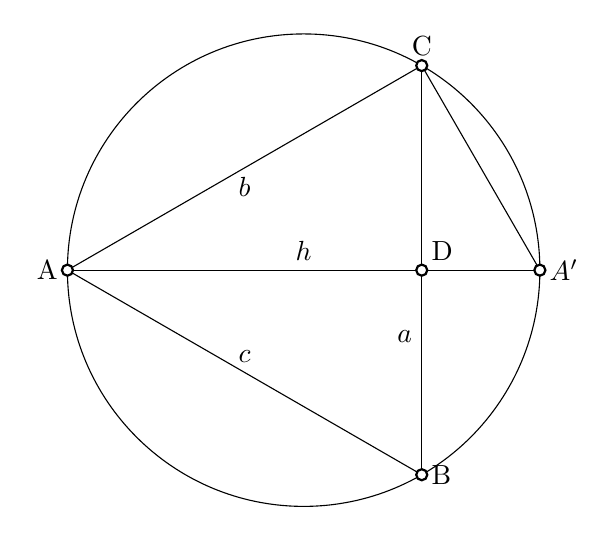
\begin{tikzpicture}
\tikzset{mypoints/.style={fill=white,draw=black,thick}}
\def\ptsize{2.0pt}
\coordinate[label=left:A] (A) at (-3,0);
\coordinate[label=right:{$A'$}] (A') at (3,0);
\coordinate[label=above:C] (C) at ({3./2},{3*sqrt(3)/2});
\coordinate[label=right:B] (B) at ({3./2},{-3*sqrt(3)/2});
\coordinate[label=above right:D] (D) at ({3./2},0);

\draw (0,0) circle (3cm);
\draw (A) -- (B) node[midway, above] {$c$};
\draw (C) -- (A');
\draw (B) -- (C) node[pos=0.3, above left] {$a$};
\draw (C) -- (A) node[midway, below] {$b$};
\draw (A') -- (A) node[midway, above] {$h$};
\fill[mypoints] (A) circle (\ptsize);
\fill[mypoints] (B) circle (\ptsize);
\fill[mypoints] (C) circle (\ptsize);
\fill[mypoints] (D) circle (\ptsize);
\fill[mypoints] (A') circle (\ptsize);
    \end{tikzpicture}
    \caption{Oppgave 2, 2008.}
  \end{center}
  \end{figure}
\end{losn}

\begin{oppg}[Oppgave 1, eksamen 2009]
  La $\R^2$ betegne det Euklidske planet.

  \begin{enumerate}[a)]
  \item La $A,B,C$ være hjørnene i trekanten $\triangle ABC$. La $A',B',C'$ være midtpunktene på henholdsvis sidene $BC,CA,AB$. Vis at trekantene $\triangle ABC$ og $\triangle A'B'C'$ er formlike.
\item Anta gitt et regulært $p$-gon med sidekanter av lengde $\ell$.  La $X$ og $Y$ være midtpunktene på to tilstøtende sidekanter. Finn lengden til linjestykket $XY$.
  \end{enumerate}
\end{oppg}

\begin{losn}
  \begin{enumerate}[a)]
  \item Den enkleste løsningen er med vektorregning. Om vi tenker oss at $A$ er origo, så skriver vi de andre punktene som vektorer fra $A$. Dermed snakker vi om  $\vec{AB}$ og $\vec{AC}$ som de to andre hjørnene. Da ser vi at $B'$ er $\frac 12 \vec{AC}$, $C'$ er $\frac 12 \vec{AB}$ og $A'$ er $\vec {AB} + \frac 12 \vec {BC}$. Dermed blir lengdene til sidene lik 
\begin{align*}
\lvert \vec{A'B'} \rvert &= \lvert \vec{AB} + \frac 12 \vec {BC} - \frac 12 {AC} \rvert \\
&= \lvert \vec{AB} + \frac 12 \vec{BC} + \frac 12 \vec {CA} \rvert
\\ &= \lvert \vec{AB} + \frac 12 \vec{BA} \rvert = \lvert \vec{AB} -\frac 12 \vec{AB} \rvert \\
&=\frac 12 \lvert \vec{AB} \rvert.
\end{align*}
Og tilsvarende for de andre sidene. Dermed er alle sidekantene i $\triangle A'B'C'$ halvparten så stor som de tilsvarende sidekantene i $\triangle ABC$, og det følger at de er formlike.

\item Denne var rar. Dette var rimelig enkelt. Finn ut hva de forskjellige vinklene i et regulært $n$-gon er, og legg merke til at svaret er halvparten av avstanden fra $X$ til $Y$. Dermed blir svaret etter litt om og men $\sin \left( (\frac 12 - \frac 1n) \pi \right) \cdot \ell/2$.
  \end{enumerate}
  \begin{figure}
\begin{center}
    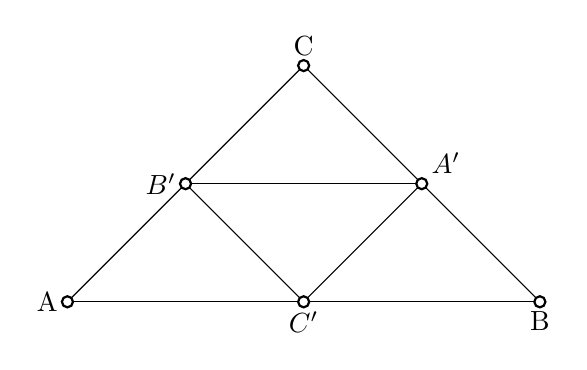
\begin{tikzpicture}
      \tikzset{mypoints/.style={fill=white,draw=black,thick}}
      \def\ptsize{2.0pt}
      \coordinate[label=left:A] (A) at (-3,0);
\coordinate[label=below:B] (B) at (3,0);
\coordinate[label=above:C] (C) at (0,3);
\coordinate[label=above right:$A'$] (A') at ({1.5},{1.5});
\coordinate[label=left:$B'$] (B') at ({-1.5},{1.5});
\coordinate[label=below:$C'$] (C') at ({0,0});
      
\draw (A) -- (B);
\draw (B) -- (C);
\draw (C) -- (A);
\draw (A') -- (B');
\draw (B') -- (C');
\draw (C') -- (A');
\foreach \p in {A,B,C,A',B',C'}
		\fill[mypoints] (\p) circle (\ptsize);
   
    \end{tikzpicture}
    \caption{Oppgave 1, 2009.}    
\end{center}
  \end{figure}
\end{losn}

\begin{oppg}
Start med en trekant $\triangle ABC$. La $\ell_A,\ell_B,\ell_C$ være linjer gjennom hjørnene $A,B,C$ som er parallele med de motstående sidene $BC,AC,AB$, henholdsvis. La $A',B',C'$ være skjæringspunktene mellom $\ell_B$ og $\ell_C$, $\ell_A$ og $\ell_C$ og $\ell_A$ og $\ell_B$, henholdsvis.
\begin{enumerate}

\item Vis at $\triangle ABC$ og $\triangle A'B'C'$ er formlike med $\triangle A'B'C'$ dobbelt så stor som $\triangle ABC$.

\item Vis at linjene $AA',BB'$ og $CC'$ er konkurrente.
\end{enumerate}
\end{oppg}

\begin{losn}
  \begin{enumerate}
  \item Vi kan bruke Figur 2 på nytt. Bare bytt om alle $A,B,C$ med $A',B',C'$ og motsatt. En vinkeljakt avslører at trekantene er formlike, og faktisk at alle fire små trekantene er formlike. Dermed følger det at hver av de små er halvparten så store (i lengder, ikke areal!) som den store.
\item Linjene $AA',BB',CC'$ er Ceva-linjer til $\triangle A'B'C'$. Da vet vi fra Cevas setning at vi vil ha
$$
\frac{B'A}{AC'} \cdot
\frac{C'B}{BA'} \cdot
\frac{A'C}{CB'} \cdot = 1
$$
Men dette er klart, fordi to og to ``halv''-sider er like lange. 
  \end{enumerate}
\end{losn}

\end{document}
